\section{Datasets}

The neural networks are trained and evaluated on 3 different datasets, KITTI\cite{kitti}, Lyft\cite{lyft2019} and Synthia. All datasets are preprocessed to remove frames where the camera is not moving. This is important because if there is no movement between frames then no depth information can be inferred during training when using monoscopic data. In the Kitti dataset the images from the left and right camera are treated as separate image sequences to yield more training data. The images are resized to 128x416 pixels, and the intrinsic camera matrix is updated accordingly. The lidar data from Kitti and Lyft is converted to sparse depth maps and are used during performance evaluation. The dataloader works by loading triplets of adjacent frames in the image sequences, and also the ground truth movement and depth map. An example of this is seen in Figure \ref{fig:sequencedataset}.

\begin{figure}[H]
	\centering
	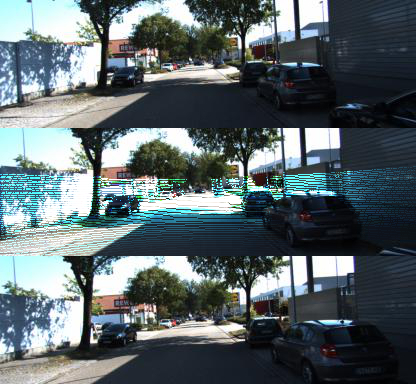
\includegraphics[width=0.5\textwidth]{sequencedataset}
	\caption{From top to bottom 3 frames from Kitti, $I_{t-1}$, $I_t$, $I_{t+1}$ with the sparse depth map overlayed on frame $I_t$.}
	\label{fig:sequencedataset}
\end{figure}

\begin{center}
	\begin{tabular}{ |c|c|c|c|c| } 
		\hline
		 &\multicolumn{2}{c|}{Sequences / Samples} \\ 
		 \hline
		 & Train & Test \\ 
		\hline
		Kitti & 110 / 16542 & 12 / 11349 \\ 
		\hline
		Lyft & 134 / 3759 & 14 / 1735 \\ 
		\hline
		Synthia & x / x & x / x \\ 
		\hline
	\end{tabular}
\end{center}


